\chapter{Introduction}

This is the RISC-V XPosit Extension draft spec. In its current state it is
merely a collection of vague ideas for how to implement posit support in RISC-V.

\section{An introduction to posits}

Posits and valids are a replacements for IEEE floats proposed by John L. Gustafson~\cite{PositArith,PositVideo,PositHub}.

The best resources for learning about posits are the following paper~\cite{PositArith} and video~\cite{PositVideo}:

\begin{itemize}
\item \url{http://www.johngustafson.net/pdfs/BeatingFloatingPoint.pdf}
\item \url{https://www.youtube.com/watch?v=N05yYbUZMSQ}
\end{itemize}

Posits represent single float-like numbers and valids are pairs of float-like numbers representing
intervals. Most of this document deals with RISC-V hardware support for posits. Hardware support
for valids are an optional feature of XPosit.

The format of a posit number is as follows:

\begin{center}
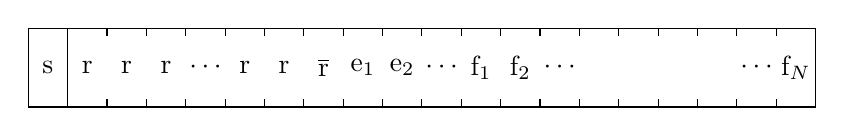
\begin{tikzpicture}
  \draw (0,0) rectangle (10,1);
  \draw[xscale=0.5,xshift=1cm] (0,0) -- (0,1.0);
  \foreach \x in {2,...,19} {
    \draw[xscale=0.5,xshift=\x cm] (0,0) -- (0,0.1) (0,0.9) -- (0,1.0);
  }
  \draw (0.25,0.5) node {s};
  \foreach \x in {0.5,1,1.5,2.5,3} {
    \draw (\x+0.25,0.5) node {r};
  }
  \draw (2.25,0.5) node {$\cdots$};
  \draw (3.75,0.5) node {$\overline{\textrm{r}}$};
  \draw (4.25,0.5) node {$\textrm{e}_1$};
  \draw (4.75,0.5) node {$\textrm{e}_2$};
  \draw (5.25,0.5) node {$\cdots$};
  \draw (5.75,0.5) node {$\textrm{f}_1$};
  \draw (6.25,0.5) node {$\textrm{f}_2$};
  \draw (6.75,0.5) node {$\cdots$};
  \draw (9.25,0.5) node {$\cdots$};
  \draw (9.75,0.5) node {$\textrm{f}_N$};
\end{tikzpicture}
\end{center}

The most significant bit is the sign bit s, followed by two or more regime bits
$\textrm{r}\textrm{r}\textrm{r}\cdots\overline{\textrm{r}}$, followed by a
configurable number of exponent bits, followed by the fraction bits (mantissa).

When the sign bit is set and all other bits are cleared then this represents the
$\pm\infty$ symbol. For valids this symbol actually represents $\pm\infty$ (with
its reciprocal being 0), but for posits it is a NaN-like token for keeping track
of domain errors.~\cite{GustafsonEmails}

When the sign bit is set and at least one other bit is set then this represents
a negative number. Decoding a negative number is done by taking the twos
complement and then decode the resulting bit pattern as the (positive) magnitude
of the negative number.

The all-zeros bit pattern represents the number zero. Note that posits do not
provide an encoding for ``negative zero''.

After the sign bit follows a variable length sequence of regime bits. A posit has
at least two regime bits. The regime bits are either a sequence of set bits
terminated by a cleared bit (zero or positive regime), or a sequence of cleared
bits terminated by a set bit (negative regime). For a zero or positive regime,
the regime $R$ is the number of leading 1 bits minus one, for a negative regime
the regime $R$ is zero minus the number of leading zero bits.

Next are the exponent bits. A Posit has $es$ exponent bits, where $es$ is a
nonnegative configuration parameter. Let $E$ be the value of the exponent.
($0 \le E < 2^{es}$)

Finally the trailing bits are the fraction bits. Like in IEEE float we
interpret them with an implicit leading 1. Let $F$ denote the fraction
value with $1 \le F < 2$.

Note that a posit may have so many regime bits that there is no space remaining
for exponent or fraction bits. In those cases the omitted bits are assumed to
be zero.

Putting it all together, the magnitute $x$ of a posit with a given $R$, $E$,
$F$, and $es$ is defined as

$$x = \left( 2^{2^{es}} \right)^R \times 2^E \times F\textrm{.}$$

The term $2^{2^{es}}$ is also referred to as ``useed''.

Posits have the following interesting properties:

\begin{itemize}
\item
  They use the bits available more efficiently than IEEE floats. Especially
  for 32-bit values and 16-bit values this can be a great advantage.
\item
  Setting $es$ enables an application to fine-tune the tradeof between dynamic
  range and precision. Usual values for $es$ are in the range $0 \le es \le 3$.
\item
  Posits have only one zero value and it is the all-zero bit pattern.
\item
  Posits have only one NaN-like value and it is a leading 1 bit followed by
  zeros, or in other words, the most negative number when interpreting the posit as a
  signed twos-complement integer ({\tt INT\_MIN}).
\item
  When $a < b$ using a signed integer interpretation, and $a \ne \texttt{INT\_MIN}$,
  then $a < b$ when interpreting the same bit pattern as posits. 
\item
  Negating a posit is just taking the twos complement.
\item
  Posits are an approximation of projective reals. They are exact in the
  horizontal direction (negation) but only approximate in the vertical
  direction (reciprocals).
\end{itemize}

\section{XPosit extension overview}

\section{Next steps}

\begin{itemize}
\item
  Transform the ideas in this proposal into a concrete RISC-V ISA
  extension.
\item
  Add hardware support for XPosit to an existing RISC-V core.
\item
  Run tests and evaluations on that implementation.
\item
  Finally propose XPosit for adoption as RISC-V standard.
\end{itemize}
